%%%%%%%%%%%%%%%%%%%%%%%%%%%%%%%%%%%%%%%%%
% Jacobs Landscape Poster
% LaTeX Template
% Version 1.1 (14/06/14)
%
% Created by:
% Computational Physics and Biophysics Group, Jacobs University
% https://teamwork.jacobs-university.de:8443/confluence/display/CoPandBiG/LaTeX+Poster
% 
% Further modified by:
% Nathaniel Johnston (nathaniel@njohnston.ca)
%
% This template has been downloaded from:
% http://www.LaTeXTemplates.com
%
% License:
% CC BY-NC-SA 3.0 (http://creativecommons.org/licenses/by-nc-sa/3.0/)
%
%%%%%%%%%%%%%%%%%%%%%%%%%%%%%%%%%%%%%%%%%

%----------------------------------------------------------------------------------------
%	PACKAGES AND OTHER DOCUMENT CONFIGURATIONS
%----------------------------------------------------------------------------------------

\documentclass[final]{beamer}

\usepackage[scale=1.2]{beamerposter} % Use the beamerposter package for laying out the poster

\usetheme{confposter} % Use the confposter theme supplied with this template

\setbeamercolor{block title}{fg=ngreen,bg=white} % Colors of the block titles
\setbeamercolor{block body}{fg=black,bg=white} % Colors of the body of blocks
\setbeamercolor{block alerted title}{fg=white,bg=dblue!70} % Colors of the highlighted block titles
\setbeamercolor{block alerted body}{fg=black,bg=dblue!10} % Colors of the body of highlighted blocks
% Many more colors are available for use in beamerthemeconfposter.sty

%-----------------------------------------------------------
% Define the column widths and overall poster size
% To set effective sepwid, onecolwid and twocolwid values, first choose how many columns you want and how much separation you want between columns
% In this template, the separation width chosen is 0.024 of the paper width and a 4-column layout
% onecolwid should therefore be (1-(# of columns+1)*sepwid)/# of columns e.g. (1-(4+1)*0.024)/4 = 0.22
% Set twocolwid to be (2*onecolwid)+sepwid = 0.464
% Set threecolwid to be (3*onecolwid)+2*sepwid = 0.708

\newlength{\sepwid}
\newlength{\onecolwid}
\newlength{\twocolwid}
\newlength{\threecolwid}
\setlength{\paperwidth}{48in} % A0 width: 46.8in
\setlength{\paperheight}{36in} % A0 height: 33.1in
\setlength{\sepwid}{0.01\paperwidth} % Separation width (white space) between columns
\setlength{\onecolwid}{0.23\paperwidth} % Width of one column
\setlength{\twocolwid}{0.464\paperwidth} % Width of two columns
\setlength{\threecolwid}{0.3\paperwidth} % Width of three columns
\setlength{\topmargin}{-0.9in} % Reduce the top margin size
%-----------------------------------------------------------

\usepackage{graphicx}  % Required for including images

% \usepackage{booktabs} % Top and bottom rules for tables

%----------------------------------------------------------------------------------------
%	TITLE SECTION 
%----------------------------------------------------------------------------------------

\title{ParkWizard: Street Parking Android App} % Poster title

\author{Siddharth Shah, Kunal Baweja, Dhruv Shekhawat, Anand Naik} % Author(s)

% \institute{\mbox{}} % Institution(s)

%----------------------------------------------------------------------------------------

\begin{document}

\addtobeamertemplate{block end}{}{\vspace*{1ex}} % White space under blocks
% \addtobeamertemplate{block alerted end}{}{\vspace*{2ex}} % White space under highlighted (alert) blocks

% \setlength{\belowcaptionskip}{2ex} % White space under figures
% \setlength\belowdisplayshortskip{2ex} % White space under equations

\begin{frame}[t] % The whole poster is enclosed in one beamer frame

\begin{columns}[t] % The whole poster consists of three major columns, the second of which is split into two columns twice - the [t] option aligns each column's content to the top

\begin{column}{\onecolwid} % The first column

%---------------
%	ABSTRACT
%--------------
\begin{alertblock}{Abstract}
A good day begins with a good parking. Finding a parking spot rather than ending up with a ticket is one of the daily struggles faced by millions of drivers worldwide, however the problem is not lack of parking, rather most of the times drivers are simply not aware of parking spots.\par
Various apps have been developed in the past but with an intention of providing paid garage parking. In this project, we introduce \textit{ParkWizard}, an user incentive based android app which crowdsources parking data and provides on demand search facility for hassle free parking.
\end{alertblock}

%------------------
%	INTRODUCTION
%------------------

\begin{block}{Introduction}
\textit{ParkWizard} is an Android app that helps users find available street parking locations. It works on a score based system where users earn points by reporting parking locations and updating availability status. The users further spend their earned score back into the app to search for available parking spots when needed. This score-based system works well towards maintaining a smooth information flow between users(drivers) who want to find available parking spots and those(informers) who have information about them. At any point, a user can update as well search for parking locations on the app.\par
\end{block}

\begin{block}{User Incentive \& Working}
\textit{Parkwizard} does not contain any parking location data of its own. It aims to incentivize users to provide the app with latest and most correct information about parking locations in their knowledge in return of earning reward points on the app. The scoring scheme is as follows:
\begin{itemize}
    \item A user is rewarded 10 points for reporting a new parking location. However, a user is not allowed to report a parking within 50m of an already existing parking to avoid duplicates.

    \item A user is rewarded 2 points for every update they provide about an already existing parking location. To limit the misuse of the update feature, we limit a user to make a maximum of 5 updates per day. These updates can be made for parking locations within 100m of the user device location.

    \item For updating false information such as suspiciously high number of parking spots or fake information, a user is penalized 2 points.

    % CONTINUED IN THIRD COLUMN
\end{itemize}

\end{block}

\end{column} % End of the first column

% Architecture
\begin{column}{\twocolwid} % The second column

\begin{block}{Algorithm}

% Algorithm Picture
\begin{figure}
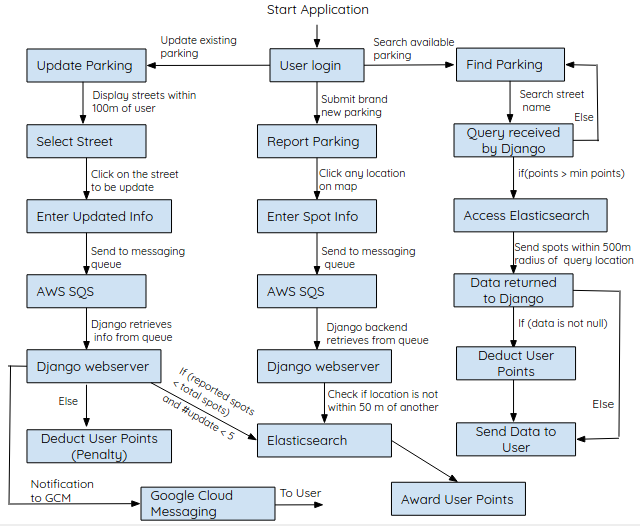
\includegraphics[width=47cm,height=40cm]{algorithm.png}
\caption{App State Transitions}
\end{figure}
\end{block}

% Vertical space hack
\vspace{1ex}

%Architecture Picture
\begin{figure}
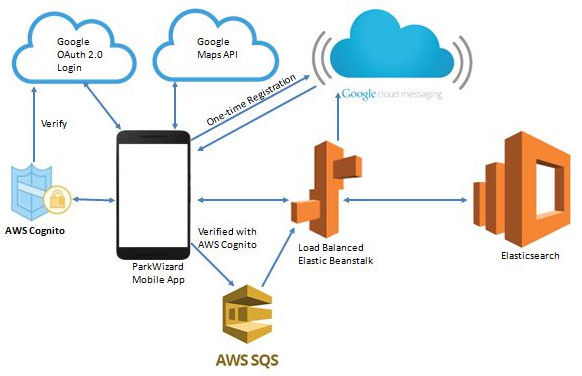
\includegraphics[width=50cm,height=29cm]{architecture_2.JPG}
\caption{Architecture}
\end{figure}

\end{column} % End of the second column

\begin{column}{\onecolwid} % The third column

\begin{itemize}
    \item A user has to spend 5 points to search for parking locations they wish to find near their destination. By default the parking locations are shown within a 500m radius of destination.

    \item To encourage users to keep the parking location most up to date, the app rewards them back 2 points if they choose to use a parking spot from the search results.
\end{itemize}

\begin{block}{Architecture}
We make use of Google OAuth to facilitate user login through Google account. At the time of login we also utilize AWS Cognito to provide users with temporary security credentials to access our app's backend resources. We have built our backend with Django webserver that communicates with Elasticsearch(ES) to store and retrieve real-time parking information. When users report parking, the information is first enqueued to SQS queue from where it is dequeued by our Django server. This ensures reliable data delivery and efficient handling of load on the server side.

On receiving the reported parking information, Django server streams it to ES which stores the data in the (lat,long, \#available spots, \#total spots) format. The user information is also stored on ES in the format (userid, points). When searching for parking, Django server retrieves the data from ES based on (lat,long) provided by user and sends it back to the app. We deploy our Django server on a load balanced AWS ElasticBeanstalk. Django server sends notifications about operation's status to Google Cloud Messaging which redirects it to the user's registered device.
\end{block}


%----------------
%	CONCLUSION
%----------------

\setbeamercolor{block alerted title}{fg=black,bg=norange} % Change the alert block title colors
\setbeamercolor{block alerted body}{fg=black,bg=white} % Change the alert block body colors

\begin{alertblock}{Conclusion}
Parkwizard is an android app with a mission to mitigate the inconvenience suffered while finding street parking. It employs a crowd-sourcing, score-based approach where users earn points on reporting free parking spots and use those points to find parking when required. ParkWizard utilizes various cloud services to function as a scalable, reliable and secure application.
\end{alertblock}

\end{column} % End of the third column

\end{columns} % End of all the columns in the poster

\end{frame} % End of the enclosing frame

\end{document}
